\chapter{Livello di trasporto}

Il livello di trasporto nella pila TCP/IP è posizionato fra il livello applicazione e il livello rete:\ fornisce quindi servizi al livello applicazione e riceve servizi dal livello rete.\
Il livello trasporto agisce da intermediario fra un programma client e il rispettivo programma server, creando un collegamento tra processi.\
Il livello trasporto è il cuore della pila TCP/IP:\ è il meccanismo end-to-end che consente di trasferire dati da un punto all'altro in Internet.

\section{Introduzione}

Il livello trasporto si colloca fra il livello rete e il livello applicazione, e fornisce un servizio di comunicazione tra processi fra i due livelli applicazione, uno sull'host locale e l'altro sull'host remoto.\
Il servizio di comunicazione viene fornito tramite una connessione logica, che consente ai due livelli applicazione (che possono essere situati in qualsiasi parte del mondo) di lavorare come se ci fosse una connessione diretta attraverso la quale inviare e ricevere i messaggi.

\subsection{I servizi del livello trasporto}

\subsubsection{\emph{Comunicazione tra processi}}

Il primo compito di un protocollo di livello trasporto è supportare la \emph{comunicazione tra processi}.\
Un processo è un'entità (programma in esecuzione) di livello applicazione che usa i servizi del livello trasporto.

Il livello rete si occupa della comunicazione tra dispositivi, ovvero della comunicazione tra host.\
Un protocollo di rete consegna i messaggi al computer destinatario, ma questo tipo di consegna è incompleta, perché i messaggi devono giungere ai processi cui erano indirizzati.\
È a questo punto che intervengono i protocolli del livello trasporto, che completano la consegna passando i messaggi ai processi applicativi destinatari.

\subsubsection{\emph{Indirizzamento:\ i numeri di porta}}

Sebbene la comunicazione tra processi possa essere realizzata in diversi modi, la più diffusa è sicuramente quella basata sul paradigma client/server.

Va osservato, però, che la maggior parte dei sistemi operativi attuali è multiutente e multiprocesso, quindi l'host locale ha spesso diversi processi client attivi, così come l'host remoto può avere diversi processi server attivi.\
Affinché si possa stabilire una comunicazione tra i due dispositivi, è necessario un metodo per individuare:\ l'host locale, l'host remoto, il processo locale e il processo remoto.\
Gli host vengono individuati per messo del loro indirizzo IP.\
I processi necessitano di ulteriori identificatori, detti \emph{numero di porta}.\
I protocolli TCP/IP usano come numeri di porta dei numeri interi compresi tra 0 e 65535 (codificabili in 16 bit).

Al client viene assegnato un numero di porta che viene detto \emph{effimero}, ovvero ``di breve durata'', dato il breve tempo di vita di un processo client.\
I numeri di porta effimeri sono superiori a 1023.

Anche al server deve essere associato un numero di porta, che, però, non può essere scelto a caso, perché tale numero deve essere in qualche modo noto al client.\
Una soluzione potrebbe essere l'invio di un pacchetto al fine di scoprire questo numero di porta, ma ciò creerebbe un carico inutile sulla rete.\
Nei protocolli TCP/IP si usano numeri universali per i server, che sono detti \emph{numeri di porta noti} (\emph{well-known}).\
Ogni client conosce il numero di porta noto del server corrispondente.

\subsubsection{\emph{Multiplexing e demultiplexing}}

Il termine \emph{multiplexing} (molti a uno) fa riferimento al caso in cui un'entità riceve informazioni da più di una sorgente; il termine \emph{demultiplexing} fa riferimento al caso in cui un'entità trasmette informazioni a più di un destinatario.\
Il livello trasporto effettua multiplexing nel sito mittente e demultiplexing nel sito destinatario.\
Le operazioni di multiplexing e demultiplexing si basano sui socket address dei processi e pertanto dipendono dal numero di porta su cui i processi sono attivi.

\paragraph{Demultiplexing senza connessione}

Lo strato di trasporto dell'host ricevente consegna il datagramma UDP alla socket identificata da IP e porta destinazione.\
I datagrammi con IP e/o porta mittente differenti ma stessi IP e porta destinatari vengono consegnati alla stessa socket.

\paragraph{Demultiplexing orientato alla connessione}

L'host ricevente usa i quattro parametri per inviare il segmento alla socket appropriata.\
Un host server può supportare più socket contemporanee (socket differenti per ogni connessione).

\section{Il protocollo TCP (Transimission Control Protocol)}

Il protocollo TCP (Transmission Control Protocol) è un protocollo orientato alla connessione e affidabile.\
Per fornire un servizio orientato alla connessione TCP prevede esplicitamente i meccanismi di apertura della connessione, di trasferimento dei dati e di chiusura della connessione.

\subsection{Servizi del protocollo TCP}

Il protocollo TCP fornisce un servizio di trasporto \emph{affidabile} tra processi basato sui numeri di porta.\
TCP effettua il multiplexing in trasmissione e il demultiplexing in ricezione.\
È un protocollo \emph{orientato alla connessione}, pertanto è necessario stabilire una connessione per ogni coppia di processi prima di avviare la comunicazione tra processi.

Quando un processo sull'host A desidera inviare e ricevere dati da un altro processo sull'host B, avvengono le seguenti tre fasi:

\begin{enumerate}
    \item I due processi TCP stabiliscono una connessione logica tra di essi.
    \item Vengono scambiati dei dati in entrambe le direzione.
    \item La connessione viene terminata.
\end{enumerate}
Si noti che si tratta di una connessione logica, non fisica.\
Il segmento TCP viene incapsulato in un datagramma IP e può essere ricevuto fuori sequenza, corrotto o addirittura smarrito e quindi ritrasmesso.\
Ciascun datagramma IP può essere instradato verso il destinatario su percorsi differenti - non esiste un collegamento fisico diretto.\
TCP crea un ambiente orientato al flusso e si occupa di consegnare al ricevente i byte nella sequenza corretta.

Oltre a essere orientato alla connessione, il protocollo TCP è anche \emph{orientato al flusso di dati} (\emph{stream-oriented}), ovvero permette al livello applicazione di trasmettere un flusso di dati.\
Un processo, quando utilizza UDP, richiede l'invio di una serie di messaggi indipendenti l'uno dall'altro.\
UDP aggiunge la propria intestazione a ciascuno di questi messaggi e li consegna al livello rete (protocollo IP) per la trasmissione.\
Ciascun messaggio del livello applicazione (prodotto da un processo in esecuzione) viene incapsulato in un pacchetto UDP che a sua volta verrà incapsulato in un datagramma IP.\
UDP e IP non riconoscono alcuna relazione fra i vari datagrammi.

TCP, al contrario, consente al processo in trasmissione di fornire i dati in un flusso continuo di byte, che viene ricevuto come tale dal processo in ricezione.\
TCP crea un ambiente nel quale i due processi sembrano essere collegati tramite un ``tubo'' che trasporta la sequenza di byte attraverso Internet.\
Il processo in trasmissione produce (immette) il flusso, mentre il processo in ricezione lo consuma (legge).

Poiché i processi in trasmissione e in ricezione non scrivono o leggono i dati necessariamente alla stessa velocità, occorrono dei buffer in cui si possano memorizzare i segmenti inviati e ricevuti.\
Vi sono due buffer, uno di trasmissione e uno di ricezione, per ciascuna direzione.\
Si vedrà nel seguito che questi buffer sono necessari anche ai meccanismi di controllo di flusso e di gestione degli errori previsti da TCP.

Sebbene la bufferizzazione possa gestire la differenza di velocità fra i processi produttore e consumatore, è necessario un passo ulteriore per poter trasmettere i dati.\
Il livello rete, quale fornitore di servizi al protocollo di livello trasporto, deve inviare i dati in pacchetti, e non come flusso di byte.\
A livello trasporto, TCP raggruppa quindi un certo numero di byte in unità chiamate \emph{segmenti}.\
TCP aggiunge un'intestazione formata da varie informazioni di controllo a ciascun segmento, che consegna al livello rete per la trasmissione.\
I segmenti vengono incapsulati in datagrammi IP e trasmessi.\
Tutte queste operazioni risultano essere perfettamente trasparenti al processo ricevente.\
Si noti che i segmenti non sono necessariamente tutti della stessa dimensione.

Un altro aspetto da considerare è che il protocollo TCP offre un servizio \emph{full-duplex}, nel quale i dati possono fluire contemporaneamente in entrambe le direzioni.\
Ciascuna entità TCP ha quindi i propri  buffer di trasmissione e ricezione e i segmenti possono circolare in entrambe le direzioni.

\subsection{Numeri di sequenza e di riscontro}

TCP per realizzare un servizio di trasporto affidabile usa un meccanismo di numerazione che prevede due campi, chiamati \emph{numero di sequenza} e \emph{numero di riscontro} (\emph{ack}).\
Questi due campi sono contenuti nell'intestazione dei segmenti TCP e fanno riferimento a un numero di byte e non a un numero di segmento.\
TCP numera ciascun byte di dati che viene trasmesso in una connessione.\
Tale numerazione è indipendente in ciascuna direzione.\
Quando TCP riceve i byte di dati da un processo, li memorizza nel buffer di trasmissione e li numera.\
La numerazione non deve necessariamente iniziare da 0 bensì da un numero arbitrario fra 0 e 2\textsuperscript{32} - 1 come indirizzo del primo byte.

TCP, dopo aver numerato i byte, assegna un numero di sequenza a ogni segmento che viene inviato.\
Il numero di sequenza, per ciascuna direzione, viene definito come segue:

\begin{enumerate}
    \item Il numero di sequenza del primo segmento, detto ISN (\emph{Initial Sequence Number} - Numero di Sequenza Iniziale), è un numero casuale.
    \item Il numero di sequenza di qualsiasi altro segmento è il numero di sequenza del segmento precedente sommato al numero di byte (reali o fittizi) ivi contenuti.
\end{enumerate}

L'intestazione dei segmenti, oltre al numero di sequenza contiene anche un numero di riscontro (acknowledgment, per brevità ack).\
Poiché la comunicazione in TCP è full-duplex, a connessione stabilita entrambe le entità possono inviare e ricevere contemporaneamente dati.\
Entrambe numerano i byte dati, in genere con un numero di partenza differente.\
Per ciascuna direzione, il numero di sequenza indica il numero del primo byte contenuto nel segmento.\
Entrambe le entità utilizzano un numero di riscontro per confermare i byte ricevuti.\
Tuttavia il numero di riscontro indica il numero del prossimo byte che l'entità si aspetta di ricevere (e non il numero dell'ultimo byte ricevuto).

\subsection{Protocolli bidirezionali}

Poiché i pacchetti dati vengono trasmessi in entrambe le direzioni, anche i riscontri devono viaggiare in entrambe le direzioni.\
Per migliorare l'efficienza dei protocolli bidirezionali viene utilizzata una tecnica chiamata \emph{piggybacking} (``viaggiare in spalla a qualcuno'').\
Quando un pacchetto trasporta dei dati da A a B, può trasportare anche i riscontri relativi ai pacchetti ricevuti da B; viceversa, quando un pacchetto trasporta dei dati da B ad A, può trasportare anche i riscontri relativi ai pacchetti ricevuti da A.

\subsection{Formato dei segmenti}

Il protocollo TCP riceve i dati in forma di messaggi dal livello applicazione e li incapsula in \emph{segmenti}.\
Il segmento consiste di un'intestazione di dimensione compresa tra i 20 e i 60 byte, seguito dai dati provenienti dal programma applicativo.\
La dimensione dell'intestazione è di 20 byte in assenza di opzioni, fino a 60 byte altrimenti.

\begin{figure}[H]
    \centering
    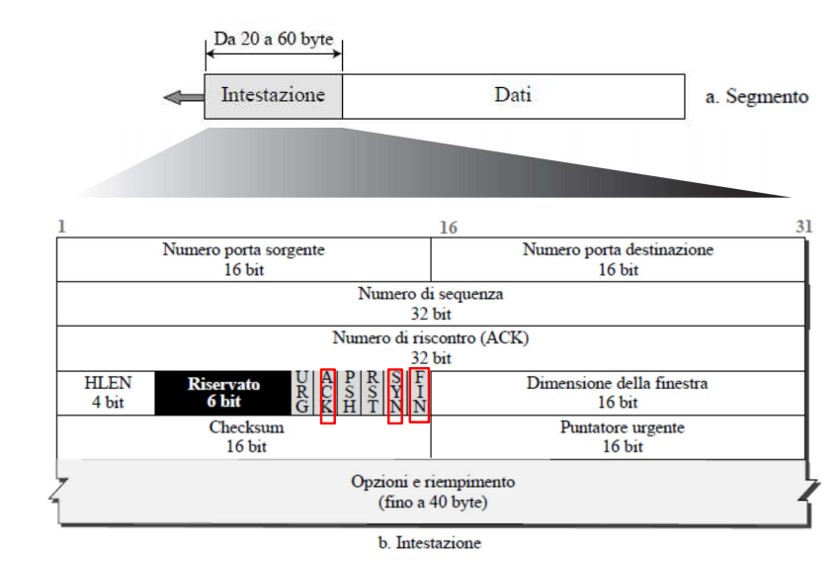
\includegraphics[width=0.8\textwidth]{immagini/SegmentoTCP.jpg}
    \caption*{Formato dei segmenti TCP}
\end{figure}

\begin{itemize}
    \item \emph{Numero di porta sorgente}.\
          Campo a sedici bit contenente il numero di porta del processo mittente sull'host che invia il segmento.
    \item \emph{Numero di porta destinazione}.\
          Campo a sedici bit contenente il numero di porta del processo destinatario sull'host che riceve il segmento.
    \item \emph{Numero di sequenza}.\
          Campo a 32 bit contenente il numero attribuito al primo byte di dati contenuto nel segmento.
    \item \emph{Numero di riscontro} (acknowledgement number).\
          Campo a 32 bit che contiene il numero di sequenza del byte che il destinatario si aspetta di ricevere.
    \item \emph{Lunghezza dell'intestazione (HLEN)}.\
          Campo a quattro bit che indica il numero di parole di quattro byte presenti nell'intestazione TCP.
    \item \emph{Flag di controllo}.\
          Campo contenente 6 bit di controllo (flag); è possibile che più di un bit sia attivo simultaneamente.
          \begin{itemize}
              \item URG:\ il campo \emph{puntatore urgente} contiene dati significativi da trasferire in via prioritaria.
              \item ACK:\ il campo \emph{numero di riscontro} contiene dati significativi
              \item PSH:\ funzione Push (trasferimento immediato dei dati in un segmento dal traporto al livello applicativo).
              \item RST:\ reset della connessione.
              \item SYN:\ sincronizza il numero di sequenza.
              \item FIN:\ non ci sono altri dati dal mittente - chiusura della connessione
          \end{itemize}
    \item \emph{Dimensione della finestra}.\
          Campo a 16 bit che indica la dimensione della finestra di cui l'altro host coinvolto nella trasmissione deve disporre.
    \item \emph{Checksum}.\
          Campo a 16 bit contenente il checksum; viene usato per il controllo degli errori.
    \item \emph{Opzioni}.\
          Vi possono essere da 0 a 40 byte di informazioni opzionali nell'intestazione del pacchetto TCP.
\end{itemize}

\subsection{La connessione TCP}

Il protocollo TCP è orientato alla connessione, ovvero stabilisce un percorso virtuale fra il mittente e il destinatario.\
Tutti i segmenti appartenenti a un messaggio vengono spediti lungo questo percorso logico.\
Utilizzare un percorso virtuale per l'intero messaggio semplifica il processo di conferma e di ritrasmissione dei segmenti smarriti o danneggiati.\
Ci si potrebbe chiedere come TCP possa essere orientato alla connessione dato che utilizza i servizi di IP, un protocollo privo di connessioni.\
In realtà la connessione TCP è virtuale, non fisica.\
TCP opera a un livello più alto:\ utilizza i servizi di IP per consegnare i singoli segmenti al destinatario, ma è il TCP stesso che controlla la connessione.\
Un segmento smarrito o danneggiato viene ritrasmesso da TCP, ma IP è inconsapevole di tale ritrasmissione.\
Un segmento ricevuto fuori sequenza viene bufferizzato da TCP fino a quando riceve il segmento mancante:\ IP è ignaro di questo riordinamento.

La trasmissione orientata alla connessione nel protocollo TCP richiede tre fasi:\ apertura della connessione, trasmissione dei dati e chiusura della connessione.

\subsubsection{\emph{Apertura della connessione}}

TCP trasmette i dati in modalità full-duplex:\ due entità TCP connesse in due macchine differenti sono in grado di trasmettere dati l'una all'altra simultaneamente.\
Questo comporta che ciascuna entità deve inizializzare la comunicazione e ottenere l'approvazione dell'entità corrispondente prima di poter trasferire qualsiasi dato.

La procedura di apertura della connessione in TCP è detta \textbf{three way handshake} (stretta di mano a tre vie).\
Consideriamo un esempio in cui un programma applicativo, chiamato client, vuole collegarsi a un altro programma applicativo, chiamato server, usando il protocollo di livello trasporto TCP.

Il processo server deve essere attivo, e pronto ad accettare connessioni mediante il livello TCP, per cui deve richiedere al TCP una \emph{apertura passiva}.\
Nonostante il server TCP sia in grado di aprire connessioni con un qualsiasi dispositivo connesso alla rete mondiale, non può aprire la connessione da solo, ma dietro la richiesta di un processo applicativo.

La richiesta fatta dal processo client, invece, è detta richiesta di \emph{apertura attiva}:\ un processo client che voglia aprire una connessione con un processo server su un particolare dispositivo ne informa il suo TCP, il quale dà inizio alla procedura three way handshake.

La procedura comporta i tre passi seguenti:
\begin{enumerate}
    \item Il client invia il primo segmento, un segmento SYN nel quale viene impostato il solo flag SYN, che serve per la sincronizzazione dei numeri di sequenza.\
          Il client sceglie un numero random come primo numero di sequenza, chiamato numero di sequenza iniziale, o ISN, e lo invia al server.\
          Si noti che questo segmento non contiene alcun numero di riscontro e non definisce la dimensione della finestra:\ quest'ultima è siginificativa solo nel caso in cui il segmento include un riscontro.\
          Si noti che il segmento SYN è un segmento di controllo e non contiene dati utente, tuttavia usa un numero di sequenza:\ quando inizierà il trasferimento dei dati, il numero di sequenza verrà incrementato di un'unità.\
          Si potrebbe dire che il segmento SYN non trasporta dati reali, ma solo un byte immaginario.
    \item Il server invia il secondo segmento, un segmento con i due flag SYN e ACK attivati.\
          Il suo scopo è duplice:\ in primo luogo è un segmento SYN per la comunicazione nell'altra direzione.\
          Il server utilizza questo segmento per inizializzare un numero di sequenza necessario per numerare i byte inviati dal server al client.\
          In un secondo luogo il server usa il segmento per riscontrare la ricezione del segmento SYN dal client impostando il flag ACK e indicando il prossimo numero di sequenza che si aspetta di ricevere dal client.\
          Dato che contiene un riscontro, deve anche definire la dimensione della finestra di ricezione (\emph{rwnd}) che il client dovrà utilizzare.\
          Essendo un segmento SYN esso deve essere confermato, quindi usa un numero di sequenza.
    \item Il client invia il terzo segmento, un segmento ACK, che conferma l'avvenuta ricezione del secondo segmento mediante il flag ACK.\
          Si noti che il segmento ACK non usa alcun numero di sequenza se non contiene dati utenti, ma alcune implementazioni consentono a questo terzo segmento, nella fase di apertura della connessione, di trasportare i primi dati dal client:\ in questo caso si deve utilizzare un numero di sequenza per indicare il numero del primo byte nei dati.
\end{enumerate}

\begin{figure}[H]
    \centering
    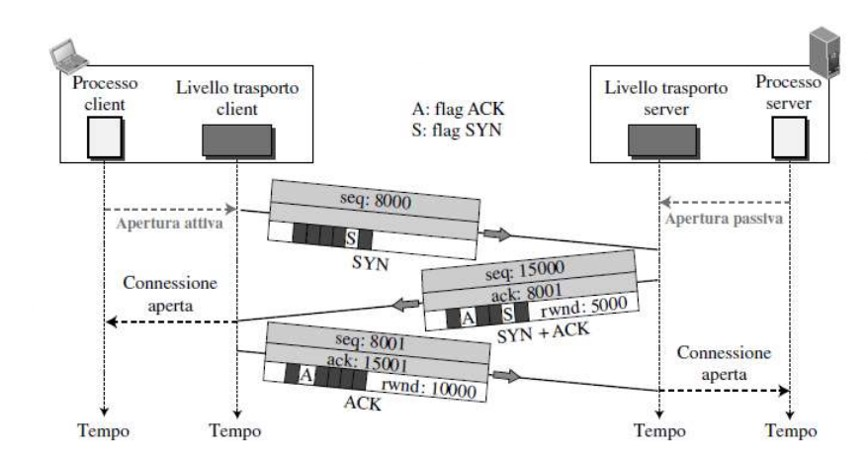
\includegraphics[width=0.8\textwidth]{immagini/3_way_open.jpg}
    \caption*{Apertura della connessione mediante il three-way handshake}
\end{figure}

\subsubsection{\emph{Chiusura della connessione}}

Ciascuna delle due parti coinvolta nello scambio dei dati (client o server) può chiudere la connessione, sebbene la chiusura sia solitamente iniziata dal client.\
La maggior parte delle implementazioni attuali fornisce due opzioni per la chiusura della connessione:\ handshake a tre vie e handshake a quattro vie con l'opzione di half-close.

\begin{enumerate}
    \item Il client TCP, dopo aver ricevuto un comando di chiusura del processo applicativo client, invia un primo segmento FIN nel quale viene impostato il flag FIN.\
          Si noti che il segmento FIN può contenere l'ultima parte dei dati inviati dal client o può essere un semplice segmento di controllo.\
          Se si tratta di un segmento di controllo, usa un solo numero di sequenza perché richiede un riscontro.
    \item Il server TCP, dopo aver ricevuto il segmento FIN, notifica la situazione al suo processo applicativo e invia il segmento FIN + ACK, per riscontrare le ricezione del segmento FIN al client e per annunciare la chiusura della connessione nella direzione opposta.\
          Questo segmento può anche contenere gli ultimi dati da parte del server; se non trasporta dati, consuma solo un numero di sequenza perché è necessario riscontrare la ricezione.
    \item Il client TCP invia l'ultimo segmento dell'handshake, un segmento ACK, per riscontrare la ricezione del segmento del segmento FIN dal server TCP.\
          Questo segmento contiene il numero di riscontro, che vale uno più il numero di sequenza ricevuto nel segmento FIN dal server; non può trasportare dati e non consuma numeri di sequenza.
\end{enumerate}
\begin{figure}[H]
    \centering
    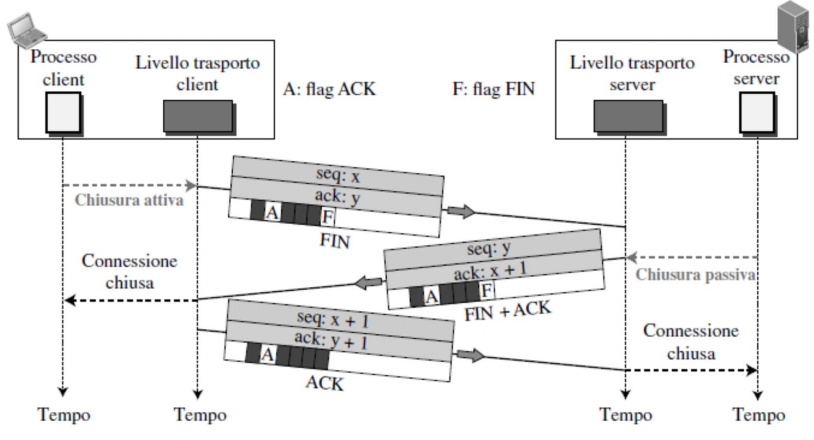
\includegraphics[width=0.8\textwidth]{immagini/3_way_close.png}
    \caption*{Chiusura della connessione mediante three-way handshake.}
\end{figure}
\textbf{\emph{Half-close}}\\
In TCP, uno dei due processi può smettere di inviare dati mentre ne sta ancora ricevendo:\ si tratta della cosidetta \emph{half-close} (chiusura a metà).\
Sebbene entrambe le entità possano eseguire la half-close, essa è solitamente iniziata dal client.\
Questo può avvenire quando il server ha bisogno di tutti i dati prima di poter procedere alla loro elaborazione.\
Un esempio classico è l'ordinamento:\ quando il client invia i dati al server affinché siano ordinati, il server deve ricevere tutti i dati prima di poter iniziare l'ordinamento.\
Il client può dunque chiudere la connessione nella direzione di uscita una volta trasmessi tutti i dati, mentre la connessione nella direzione di ingresso deve rimanere aperta per poter ricevere i risultati.\
Il server, dopo aver ricevuto i dati, ha bisogno di più tempo per poterli ordinare, la sua connessione in uscita deve quindi rimanere aperta.

Il client chiede l'half-close della connessione inviando un segmento FIN.\
Il server accetta la richiesta di chiusura inviando un segmento ACK.\
Il trasferimento dei dati dal client al server termina, ma il server può continuare a inviare dati.\
Quando il server ha terminato l'invio dei dati elaborati, invia un segmento FIN, che viene riscontrato da un segmento ACK dal client.

Dopo il completamento della half-close è ancora possibile trasmettere i dati dal server al client e i riscontri dal client al server, ma il client non può inviare altri dati.

\paragraph{Stato TIME-WAIT}

TIME-WAIT è lo stato finale in cui il capo di una connessione che esegue la chiusura attiva resta prima di passare alla chiusura definitiva della connessione.\
Il tempo di permanenza in questo stato è di 2MSL.

La MSL è la \emph{stima del massimo periodo di tempo che un pacchetto IP può vivere sulla rete}; questo tempo è limitato perché ogni pacchetto IP può essere ritrasmesso dai router un numero massimo di volte (detto hop limit).

\begin{figure}[H]
    \centering
    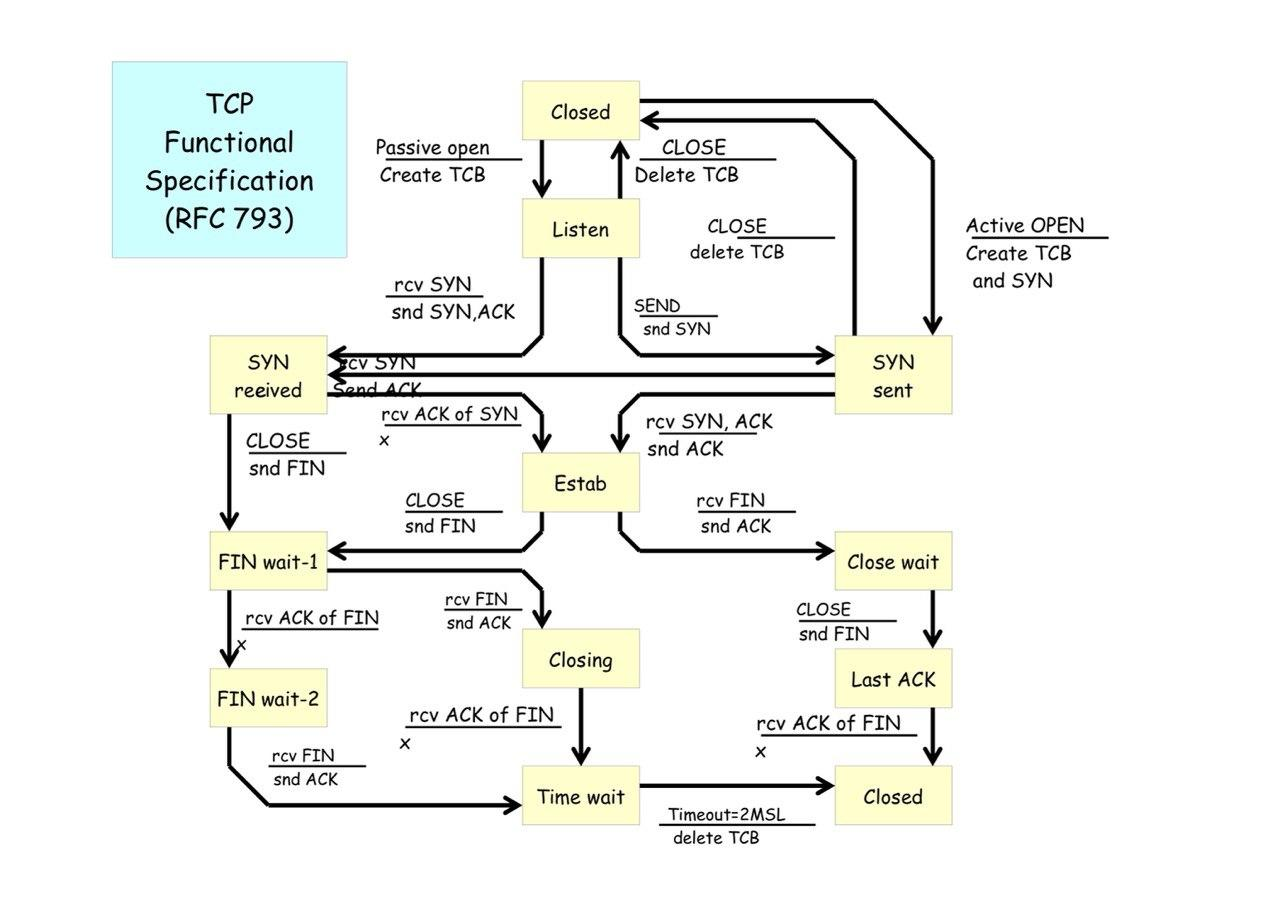
\includegraphics[width=0.9\textwidth]{immagini/Diagramma.jpg}
    \caption*{Diagramma delle transizioni di stato}
\end{figure}

Lo stato TIME-WAIT viene utilizzato dal protocollo per due motivi principali:
\begin{itemize}
    \item \textbf{implementare in maniera affidabile la terminazione della connessione} in entrambe le direzioni
          \begin{itemize}
              \item Se l'ultimo ACK della sequenza viene perso, chi esegue la chiusura passiva manderà un ulteriore FIN, chi esegue la chiusura attiva deve mantenere lo stato della connessione per poter reinviare l'ACK.
          \end{itemize}
    \item \textbf{consentire l'eliminazione dei segmenti duplicati in rete}
\end{itemize}

\begin{table}[H]
    \centering
    \begin{tabular}{|l|m{22em}|}
        \hline
        \emph{Stato} & \emph{Descrizione}                                                                                \\
        \hline
        CLOSED       & Assenza di connessione.                                                                           \\
        \hline
        LISTEN       & Ricevuta richiesta di apertura passiva; server in attesa di un messaggio SYN da parte del client. \\
        \hline
        SYN-SENT     & Richiesta di connessione SYN inviata, in attesa di ACK.                                           \\
        \hline
        SYN-RCVD     & SYN + ACK inviati; in attesa di ACK.                                                              \\
        \hline
        ESTABLISHED  & Connessione aperta, trasferimento dati in atto.                                                   \\
        \hline
        FIN-WAIT-1   & Primo FIN inviato; in attesa di ACK.                                                              \\
        \hline
        FIN-WAIT-2   & Ricevuto ACK al primo FIN; in attesa di secondo FIN.                                              \\
        \hline
        CLOSE-WAIT   & Ricevuto primo FIN, ACK inviato; in attesa che il processo richieda la chiusura.                  \\
        \hline
        TIME-WAIT    & Ricevuto secondo FIN, ACK inviato, in attesa del timeout 2MSL.                                    \\
        \hline
        LAST-ACK     & Secondo FIN inviato; server in attesa di ACK.                                                     \\
        \hline
        CLOSING      & Le due parti hanno deciso simultaneamente di chiudere la connessione                              \\
        \hline
    \end{tabular}
    \caption*{Stati del protocollo TCP}

\end{table}

\subsection{Controllo degli errori}

Il protocollo TCP è un protocollo di trasporto affidabile; ovvero garantisce al livello applicazione che i dati inviati verranno consegnati nel giusto ordine, senza errori, senza smarrimenti o duplicazioni.

Il controllo degli errori garantisce affidabilità e prevede meccanismi per l'individuazione e la rispedizione dei segmenti corrotti, per la rispedizione dei segmenti smarriti, per l'identificazione e lo scarto dei segmenti duplicati e per la memorizzazione dei segmenti ricevuti fuori sequenza fino a quando non arrivano i segmenti mancanti.\
I tre semplici strumenti usati dal protocollo TCP per individuare gli errori di trasmissione sono il checksum, i messaggi di riscontro e il timeout.

\subsubsection{\emph{Checksum}}

Il protocollo TCP prevede che ciascun segmento contenga un campo checksum di 16 bit, utilizzato per identificare i segmenti corrotti.\
Se un segmento è corrotto, questo viene ignorato dal destinatario e considerato smarrito.\
TCP utilizza un checksum di 16 bit, obbligatorio in ogni segmento.

\subsubsection{\emph{Riscontri}}

TCP utilizza i riscontri per confermare la ricezione dei segmenti dati e dei segmenti di controllo che non contengono dati ma che usano un numero di sequenza.\
I segmenti di riscontro (ACK) non sono mai riscontrati.

Il protocollo TCP è stato originariamente progettato per riscontrare la ricezione dei segmenti in modo cumulativo:\ il destinatario notifica il numero di byte che si attende, ignorando tutti gli eventuali segmenti giunti fuori sequenza e memorizzati.\
Questa tecnica viene a volte indicata come \emph{riscontro cumulativo positivo} (ACK).\
Il termine positivo si riferisce al fatto che i segmenti scartati, smarriti o duplicati non vengono notificati.\
Il campo ACK a 32 bit nell'intestazione TCP è utilizzato per i riscontri cumulativi e il suo valore è da considerarsi valido solo quando è impostato il flag corrispondente ACK.

Un numero crescente di implementazioni stanno aggiungendo un nuovo tipo di riscontro chiamato \emph{selettivo} (SACK).\
Il SACK non sostituisce l'ACK, ma notifica ulteriori informazioni al mittente:\ segmenti che non sono in sequenza e segmenti duplicati.\
Tuttavia, dato che non è possibile aggiungere questo tipo di informazioni nell'intestazione TCP, SACK viene implementato come opzione al teminine dell'intestazione.

Quando, il destinatario, genera i riscontri? Nell'evoluzione di TCP sono state definite varie regole, utilizzate poi da varie implementazioni.\
Di seguito si riportano le regole più comuni; l'ordine non riflette necessariamente l'importanza.

\begin{enumerate}
    \item Quando un'entità invia un segmento dati all'entità corrispondente, deve includere (piggybacking) un riscontro che fornisca il prossimo numero di byte che prevede di ricevere.\
          Questa regola diminuisce il numero di segmenti necessari e riduce quindi il traffico.
    \item Quando il destinatario non ha dati da inviare e riceve un segmento nell'ordine corretto (ovvero con il numero di sequenza atteso) e il segmento precedente è già stato riscontrato, ritarda l'invio del segmento ACK fino a quando non arriva un altro segmento o fino a quando non scade un tempo massimo predefinito (normalmente di 500 ms).\
          In altre parole il destinatario ritarda l'invio di un segmento ACK se ha un unico segmento nella sequenza corretta da riscontrare.\
          Anche questa regola (detta \emph{ACK posticipato} o \emph{delayed}) evita che i segmenti ACK creino un traffico eccessivo, e fa uso di un timer di ACK-posticipato.
    \item Quando arriva un segmento con numero di sequenza atteso e il segmento precedente non è stato riscontrato, il destinatario invia immediatamente un segmento ACK.\
          In altre parole, non ci devono mai essere più di due segmenti nell'ordine corretto non riscontrati.\
          Questo serve a evitare l'inutile ritrasmissione dei segmenti, che potrebbe produrre congestione nella rete.
    \item Quando arriva un segmento fuori sequenza, il destinatario invia immediatamente un segmento ACK notificando il numero di sequenza atteso nel prossimo segmento.\
          Questo consente la \emph{ritrasmissione rapida} (fast retransmission) di eventuali segmenti smarriti.
    \item Quando arriva un segmento mancante, il destinatario invia un segmento ACK per notificare il prossimo numero di sequenza atteso.\
          Questo serve a notificare al mittente l'avvenuta ricezione di un segmento precedentemente annunciato come smarrito.
    \item Quando arriva un segmento duplicato, il destinatario lo scarta e invia immediatamente un riscontro con il numero di sequenza del prossimo segmento atteso.\
          Questo risolve alcuni problemi legati alla perdita dei segmenti di conferma.
\end{enumerate}

\subsubsection{\emph{Ritrasmissione dei segmenti}}

Il cuore del meccanismo di controllo degli errori è la ritrasmissione dei segmenti:\ quando un segmento viene inviato, viene memorizzato in una coda in attesa di essere riscontrato.\
Alla scadenza del timer di ritrasmissione o quando il mittente riceve tre ACK duplicati per il precedente segmento nella coda, quel segmento viene trasmesso.\
Analizziamo ora i due casi nel dettaglio.\

Il TCP mittente inizializza un \emph{timer di ritrasmissione} o RTO (Retransmission Time-Out), per ogni segmento inviato.\
Allo scadere del tempo limite senza averne ricevuto un riscontro, il segmento all'inizio della coda (il segmento con il numero di sequenza inferiore) viene ritrasmesso e si fa ripartire il timer.\
Si noti che si ipotizza sempre che $S_f<S_n$, dove S\textsubscript{f} (\emph{SendFirst}) è il numero di sequenza del primo byte in attesa di essere riscontrato e S\textsubscript{n}(\emph{Send next}) è il prossimo byte da inviare.

La regola relativa alla trasmissione dei segmenti è sufficiente se il valore RTO non è eccessivo.\
A volte, tuttavia, viene smarrito un segmento e il destinatario riceve un numero tanto elevato di segmenti fuori sequenza da non poterli memorizzare (per la dimensione limitata del buffer).\
Per risolvere questo problema, la maggior parte delle implementazioni attuali osservano la regola dei \emph{tre ACK duplicati} e ritrasmettono immediatamente il segmento mancante.\
Questa funzione viene chiamata \emph{ritrasmissione veloce}.\
Con questa versione quando vengono ricevuti tre ACK duplicati (ovvero l'ACK originale più tre copie identiche) di un segmento, quello successivo viene immediatamente ritrasmesso senza attendere il timeout.

Quando un segmento viene ritardato, smarrito o scartato, i segmenti che lo seguono giungono fuori sequenza (non nell'ordine atteso).\
La maggior parte delle implementazioni attuali del TCP non scartano i segmenti fuori sequenza, ma li memorizzano temporaneamente in attesa di ricevere il segmento mancante.\
Si noti tuttavia che i segmenti fuori sequenza non possono essere trasmessi al processo, dato che TPC garantisce la consegna dei dati nell'ordine corretto.

\subsubsection{Calcolo del timeout}

Il tempo di timeout (RTO) è fondamentale per il funzionamento di TCP.\
Deve essere maggiore di RTT (Round Trip Time):\ tempo trascorso da quando si invia un segmento a quando se ne riceve il riscontro.\
Viene calcolato analizzando gli RTT dei segmenti non ritrasmessi (Sample RTT, stimato per un segmento trasmesso - non per ogni invio).

\begin{center}
    $RTT_{ESTIMATED} = (1-\alpha) \cdot RTT_{ESTIMATED} + \alpha \cdot RTT_{SAMPLE}$
\end{center}
RTT\textsubscript{SAMPLE} può fluttuare.\
Si considera RTT\textsubscript{ESTIMATED} come la combinazione dei precedenti valori di RTT\textsubscript{ESTIMATED} con il nuovo valore RTT\textsubscript{SAMPLE}.\
Il valore di $\alpha $ viene posto a 1/8 in modo da rendere via via meno importanti gli RTT dei pacchetti più vecchi (RFC 2988).

\begin{center}
    $RTT_{ESTIMATED} = 0,875 \cdot RTT_{ESTIMATED} + 0,125 \cdot RTT_{SAMPLE}$
\end{center}

Oltre al valore RTT stimato è necessario anche una stima della variabilità di RTT data dalla seguente formula

\begin{center}
    $RTT_{DEV} = (1-\beta)RTT_{DEV} + \beta|RTT_{SAMPLE} - RTT_{ESTIMATED}|$
\end{center}
Stima di quanto RTT\textsubscript{SAMPLE} si discosta da RTT\textsubscript{ESTIMATED}.\
Il valore $\beta$ viene posto a 1/4 (RFC 2988).

Una volta ottenuti questi valori, il timeout viene normalmente calcolato come

\begin{center}
    $RTO = RTT_{ESTIMATED} + 4RTT_{DEV}$
\end{center}
In molte implementazioni, dopo un errore (es.\
ACK non ricevuto) si raddoppia il timeout:\ si tratta di un primo meccanismo di controllo della congestione.

\subsubsection{\emph{Alcuni scenari}}

\paragraph{\emph{Operatività normale}}

Il primo scenario illustra il trasferimento di dati bidirezionali fra due sistemi.\
Il client TCP invia un segmento, il server TCP ne invia tre.\
Per il primo segmento del client e tutti e tre i segmenti del server si applica la prima regola:\ vi sono dati da inviare, quindi il segmento indica il prossimo byte atteso.\
Quando il client riceve il primo segmento dal server, non ha altri dati da inviare:\ invia dunque un segmento ACK.\
Tuttavia la seconda regola stabilisce che il riscontro sia ritardato (posticipato) di 500 ms in attesa di eventuali altri segmenti.\
Alla scadenza del timer viene inviata la conferma, dato che il client non può sapere se stanno arrivando altri segmenti e non può ritardare indefinitamente il riscontro.\
All'arrivo del segmento successivo viene inizializzato un altro timer di ACK-posticipato.\
Questa volta, prima che scada il tempo impostato, arriva il terzo segmento che comporta l'invio del riscontro in conformità alla terza regola.\
Il timer RTO non è stato considerato, poiché nessun segmento è stato smarrito o ritardato.\
Si assume semplicemente che il timer RTO sia gestito correttamente.

\paragraph{\emph{Segmento smarrito}}

In questo scenario si illustra il caso in cui un segmento viene smarrito o corrotto.\
I casi di segmento smarrito o corretto vengono trattati nello stesso modo dal destinatario:\ il segmento smarrito viene perso da qualche parte nella rete, il segmento corrotto viene eliminato dal destinatario stesso.\
Entrambi vengono considerati persi.\
Si suppone che il trasferimento di dati sia unidirezionale:\ una postazione trasmette, l'altra riceve.\
In questo scenario il mittente invia i segmenti 1 e 2 che sono immediatamente riscontrati con un ACK (regola 3).\
Il terzo segmento viene smarrito.\
Il destinatario riceve il segmento 4 che risulta fuori sequenza:\ ne memorizza i dati nel suo buffer ma lascia uno spazio per indicare che non vi è continuità nei dati.\
Invia immediatamente un riscontro al mittente indicando il prossimo byte atteso (regola 4).\
Si noti che l'entità TCP destinataria consegna al processo applicativo solo dati correttamente ordinati.\

Il TCP mittente mantiene un timer RTO per tutto il periodo di connessione.\
Alla scadenza del timer il TCP mittente ritrasmette il segmento 3, che questa volta arriva correttamente e viene riscontrato (regola 5).

\paragraph{\emph{Ritrasmissione veloce}}

In questo scenario si vuole esemplificare il concetto di \emph{ritrasmissione veloce}.\
Questo scenario è simile al precedente ad eccezione del valore RTO che in questo caso è superiore.

Quando il destinatario riceve un qualsiasi segmento successivo a quello atteso (in questo caso il terzo segmento) invia il riscontro indicante il segmento atteso (regola 4).\
Il mittente riceve quattro riscontri con il medesimo valore (tre duplicati).\
Sebbene il timer non sia ancora scaduto, la regola di ritrasmissione veloce richiede che il segmento 3, il segmento indicato come atteso da tutti e quattro i riscontri, sia immediatamente ritrasmesso.\
Una volta ritrasmesso il segmento, il timer viene fatto ripartire.

\paragraph{\emph{Correzione automatica di un ACK smarrito}}

Questo scenario illustra il caso in cui un riscontro smarrito viene automaticamente rimpiazzato dal successivo.\
Con la tecnica di riscontro cumulativo utilizzata dal TCP, la perdita di una conferma può passare inosservata al TCP mittente:\ il riscontro successivo corregge automaticamente lo smarrimento del riscontro.

\paragraph{\emph{Riscontro smarrito corretto con la rispedizione del segmento}}

Se il riscontro successivo subisce un lungo ritardo o non vi è riscontro successivo (il riscontro smarrito è l'ultimo), il timer RTO scade senza che si sia ricevuto alcun riscontro.\
Il mittente ritrasmette quindi il segmento, che risulta duplicato.\
Il destinatario ignora il segmento che riceve duplicato ma ritrasmette immediatamente l'ultimo ACK per informare il mittente che il segmento o i segmenti sono arrivati a buon fine.

Si noti che viene ritrasmesso solo un segmento sebbene due segmenti non siano stati riscontrati.\
Il mittente, alla ricezione dell'ACK ritrasmesso, capisce che entrambi i segmenti sono stati ricevuti correttamente dato che il riscontro è cumulativo.

\begin{figure}[H]
    \centering
    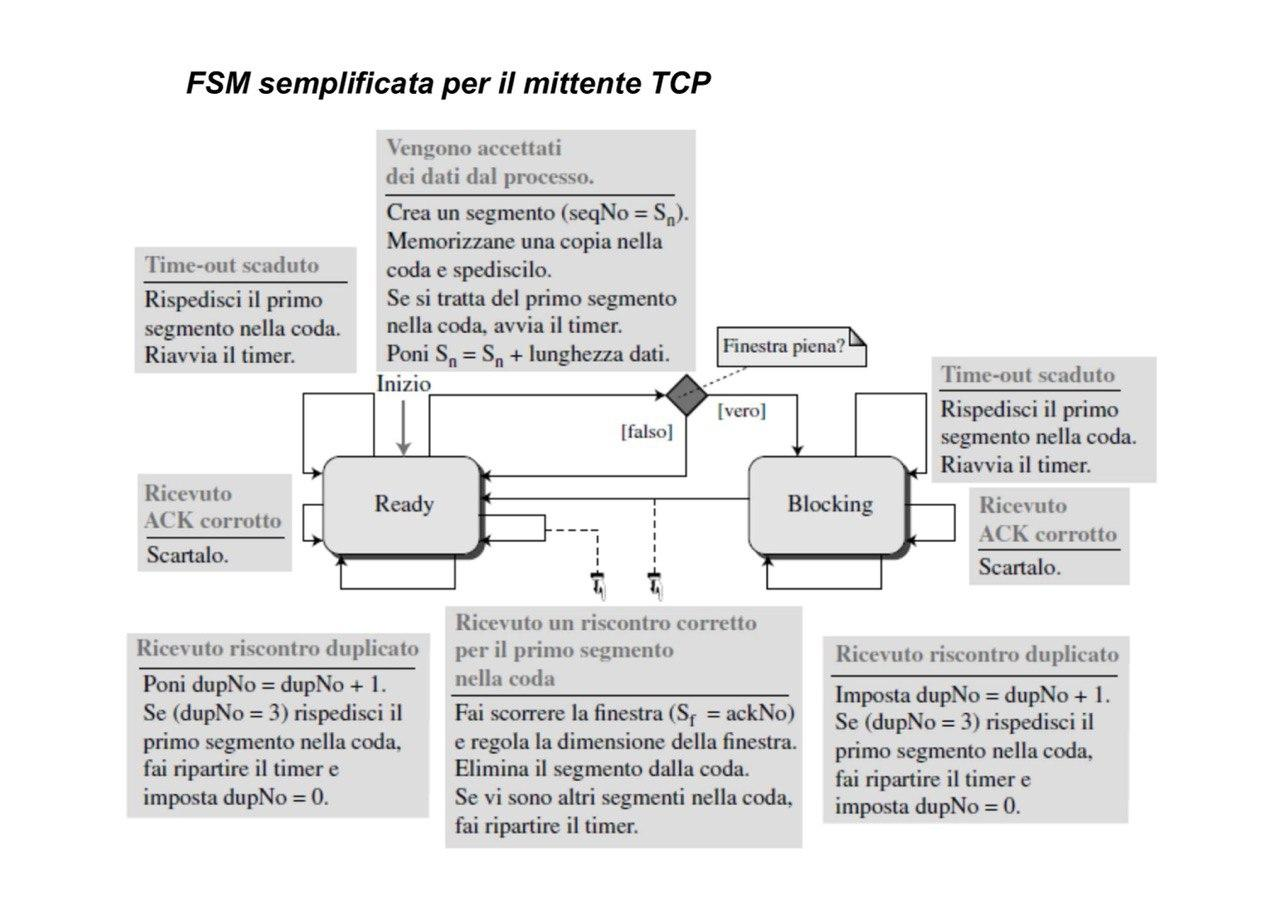
\includegraphics[width=0.9\textwidth]{immagini/FSMmittente.jpg}
\end{figure}

\begin{figure}[H]
    \centering
    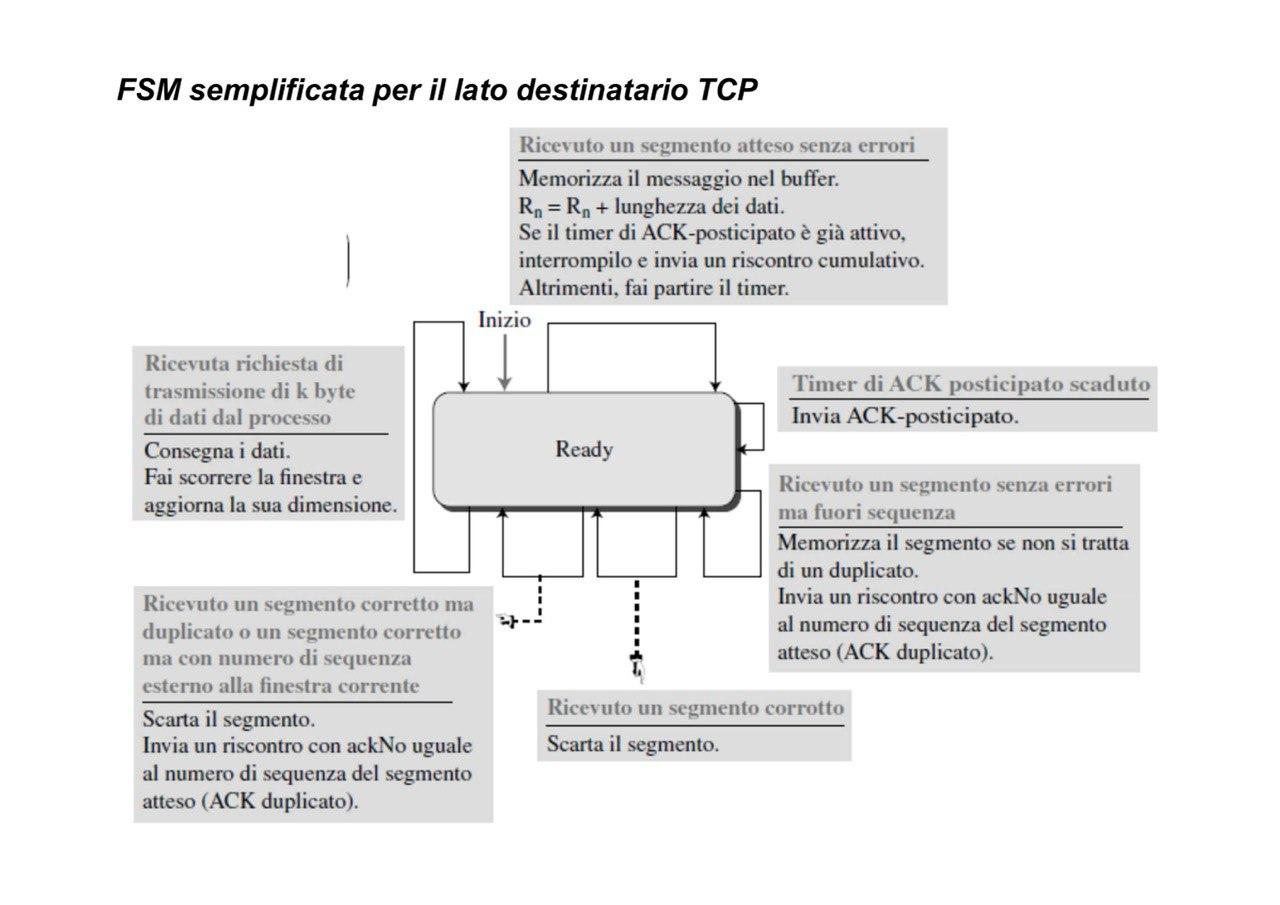
\includegraphics[width=0.9\textwidth]{immagini/FSMdestinatario.jpg}
\end{figure}

\subsection{Finestra di trasmissione}

I dati inviati dal processo a livello applicativo sono mantenuti nel buffer di invio.

La trasmissione dei dati si basa sulla finestra di trasmissione (\emph{sliding window}).
\begin{itemize}
    \item finestra sovrapposta sulla sequenze da trasmettere
    \item negoziata dinamicamente
    \item viene fatta avanzare alla ricezione di un ACK.
\end{itemize}

\begin{figure}[H]
    \centering
    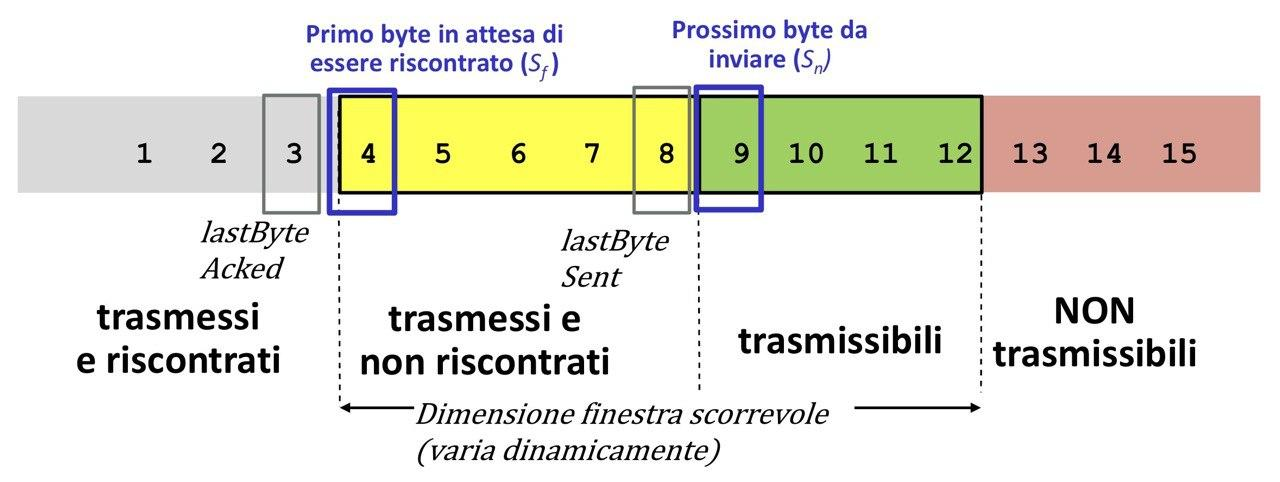
\includegraphics[width=0.6\textwidth]{immagini/Finestra_di_trasmissione.jpg}
    \caption*{Finestra di trasmissione}
\end{figure}

\subsection{Controllo di flusso}

Il \emph{controllo di flusso} consente di bilanciare la velocità con cui un produttore genera i dati con la velocità con la quale un consumatore li utilizza.\
Il protocollo TCP separa il controllo di flusso dal controllo degli errori; in questo paragrafo si descrive il controllo del flusso astraendo dal controllo degli errori:\ si assume dunque che il canale logico fra il mittente e il destinatario TCP sia di errori.

I dati generati dal processo applicativo mittente vengono prima passati (pushed) al TCP mittente, da questo trasmessi al TCP destinatario e infine da quest'ultimo al processo applicativo ricevente.\
I feedback del controllo di flusso, invece, vengono trasmessi dal TCP ricevente al TCP mittente e da questo al processo applicativo mittente.\
La maggior parte delle implementazioni TCP non fornisce feedback del flusso di controllo dal processo destinatario al TCP destinatario, ma consente al processo destinatario di richiedere a suo piacimento i dati dal TCP destinatario.\
In altri termini il TCP destinatario controlla il TCP mittente, il quale a sua volta controlla il processo mittente.

Il feedback del controllo di flusso dal TCP mittente al processo applicativo mittente è ottenuto tramite il semplice rifiuto dei dati da parte del TCP mittente quando la sua finestra è completa.\
La descrizione del controllo di flusso si concentra quindi sul feedback inviato dal TCP destinatario al TCP mittente.

\vspace{12pt}

\noindent Ogni host imposta buffer di invio e di ricezione.\
Il processo applicativo destinatario legge i dati dal buffer di ricezione (non necessariamente nell'istante in cui arrivano).\
Si intende con controllo di flusso la capacità del mittente di evitare la possibilità di saturare il buffer del ricevitore:\ mette in relazione la frequenza di invio del mittente con la frequenza di lettura dell'applicazione ricevente.

TCP implementa questa caratteristica tramite una variabile detta \textbf{finestra di ricezione} (\textbf{\emph{rwnd}}) mantenuta nel mittente:\ questa variabile fornisce un'idea di quanto spazio è ancora a disposizione nel buffer del ricevitore.\
Tale valore è comunicato nel campo window dell'header TCP.

Spazio disponibile nel buffer del destinatario

\begin{center}
    $rwnd=RcvBuffer - (LastByteReceived - LastByteRead)$
\end{center}
\emph{rwnd} è dinamica.\
L'host destinatario comunica la dimensione di \emph{rwnd} al mittente.

Il mittente si assicura che
\begin{center}
    $LastByteSent-LastByteAcked < rwnd$
\end{center}
quantità di dati trasmessi e non ancora riscontrati.

N.B.\
se $rwnd=0$, il mittente manda segmenti ``sonda'' di 1 byte per ricevere l'aggiornamento sulla dimensione di rwnd.

\subsection{Controllo della congestione in TCP}

\subsubsection{\emph{Finestra di congestione}}

Quando si è descritto il controllo di flusso nel protocollo TCP, si è detto che la dimensione della finestra di invio è controllata dal destinatario tramite il valore \emph{rwnd}, che viene indicato in ogni segmento trasmesso nella direzione opposta.\
L'impiego di questa strategia garantisce che la finestra del ricevente non venga mai sovraccaricata con i dati ricevuti.\
Questo tuttavia non garantisce che i buffer intermedi, i buffer nei router, non si congestionino.\
Un router potrebbe ricevere dati da più di un mittente.\
Indipendentemente dalla capacità del buffer di un router, è sempre possibile che questo venga saturato e che si trovi costretto a scartare i segmenti di qualche specifico mittente TCP.\
In altre parole non vi è congestione agli estremi, ma vi può essere congestione nei nodi intermedi.\
TCP deve preoccuparsi della possibile congestione della rete poiché la perdita di un gran numero di segmenti può influire significativamente sul meccanismo di controllo degli errori.\
La perdita di numerosi segmenti comporta la loro rispedizione, peggiorando così la congestione della rete e portando alla fine al collasso della comunicazione.

TCP è un protocollo end-to-end che sfrutta i servizi di IP.\
La congestione nei router è un problema che riguarda IP e che dovrebbe essere gestito a livello rete.\
Tuttavia IP è un semplice protocollo senza controllo della congestione.\
TCP è dunque necessariamente costretto a occuparsi del problema.

TCP non può ignorare la congestione nella rete:\ non può inviare un numero di segmenti eccessivo alla rete, altrimenti ne verrebbe penalizzato.\
Ma TCP non può nemmeno essere troppo conservativo, nel senso di inviare un numero troppo limitato di segmenti nell'unità di tempo, poiché non sfrutterebbe al meglio la capacità della rete.\
TCP deve quindi prevedere delle strategie per accelerare la trasmissione dei dati quando non vi è congestione e ridurre la trasmissione quando rileva la congestione.

Per controllare il numero di segmenti da trasmettere, TCP utilizza una seconda variabile chiamata \emph{cwnd} (\emph{congestion window - finestra di congestione}), il cui valore dipende dal livello di congestione nella rete.\
Le due variabili \emph{cwnd} e \emph{rwnd} congiuntamente definiscono la dimensione della finestra di invio di TCP.\
La prima variabile è legata alla congestione della rete, la seconda alla congestione delle postazioni terminali.\
La dimensione finale della finestra corrisponde al minimo dei due valori.

\begin{center}
    \textbf{Dimensione della finestra} $= \min(rwnd, cwnd)$
\end{center}

\subsubsection{\emph{Rilevare la congestione}}

Prima di analizzare come il valore di \emph{cwnd} debba essere impostato e aggiornato, è necessario descrivere come un mittente TCP possa identificare il possibile verificarsi della congestione nella rete.\
Il mittente interpreta come sintomi di congestione due eventi:\ il timeout e la ricezione di tre riscontri duplicati.

Il primo evento è dunque il \emph{timeout}.\
Se un mittente TCP non riceve un riscontro per un segmento o un gruppo di segmenti prima dello scadere del timeout, suppone che tale segmento o i segmenti siano stati smarriti a causa della congestione.

Il secondo evento è la ricezione di \emph{tre riscontri duplicati} (quattro ACK con il medesimo numero di ritorno).\
Si ricordi che un destinatario TCP invia un riscontro duplicato per segnalare un ritardo nella ricezione di un segmento, ma tre riscontri duplicati sono un'indicazione di segmento smarrito, che può essere dovuto alla congestione nella rete.\
La congestione nel caso dei tre riscontri duplicati, significa che un segmento è stato smarrito, ma anche che altri tre segmenti sono stati ricevuti:\ la rete è al limite della congestione o è appena rientrata da una congestione.

È interessante notare che il mittente TCP usa solo un tipo di feedback dal destinatario per rilevare la congestione:\ i riscontri.\
L'assenza della ricezione rapida e regolare dei riscontri, evidenziata dallo scadere del timeout, è il sintomo di una congestione severa; la ricezione di tre riscontri duplicati è il sintomo di una congestione debole.

\subsubsection{\emph{Le strategie di gestione della congestione}}

La strategia generale del protocollo TCP per gestire la congestione si basa su tre fasi:\ \emph{slow start} (partenza lenta), \emph{congestion avoidance} (prevenzione della congestione) e \emph{fast recovery} (recupero veloce).

\paragraph{\emph{Slow start:\ incremento esponenziale}}

L'algoritmo \emph{slow start} (partenza lenta) si basa sull'idea che la dimensione della finestra di congestione (\emph{cwnd}) viene inizializzata con la dimensione del segmento massimale (MSS, Maximum Segment Size), ma viene aumentata di un valore corrispondente a MSS a ogni segmento riscontrato.

Il nome dell'algoritmo è decisamente fuorviante:\ l'algoritmo parte lentamente ma procede con velocità esponenzialmente crescente.\
Si supponga che \emph{rwnd} sia molto più elevato di \emph{cwnd}, in modo tale che la finestra del mittente sia sempre uguale a \emph{cwnd}.\
Si ipotizza anche che tutti i segmenti siano della stessa dimensione di MSS byte.\
Per semplicità si ignora anche la strategia dei riscontri in ritardo e si ipotizza che ogni segmento sia riscontrato individualmente.

Il mittente inzia con $cwnd = 1$, quindi può inviare un solo segmento.\
Ricevuto il primo riscontro, il segmento riscontrato viene eliminato dalla finestra di invio:\ nella finestra si è quindi liberato spazio per un segmento.\
Anche la dimensione della finestra di congestione è incrementata di 1 perché la ricezione del riscontro è un buon sintomo di assenza di congestione nella rete.\
La dimesione della finestra vale ora 2 ed è possibile inviare due segmenti.\
Quando questi vengono confermati, la dimensione della finestra viene aumentata di 1 per ciascun riscontro ricevuto, quindi \emph{cwnd} vale ora 4 e così via.\
In altri termini, la dimensione della finestra di congestione con questo algoritmo è una funzione del numero di riscontri ricevuti e può essere determinata come segue:

\begin{center}
    Se arriva un riscontro, $cwnd = cwnd +1$
\end{center}

Valutando la dimensione di \emph{cwnd} in funzione del tempo di andata e ritorno (RTT), si trova che la velocità di crescita è esponenziale, dunque molto aggressiva, in termini di ciascun RTT:
\begin{table}[H]
    \centering
    \begin{tabular}{l c l}
        Inizio     & $\rightarrow$ & $cwnd = 1 \rightarrow 2^0$          \\
        Dopo 1 RTT & $\rightarrow$ & $cwnd=cwnd+1=1+1=2 \rightarrow 2^1$ \\
        Dopo 2 RTT & $\rightarrow$ & $cwnd=cwnd+2=2+2=4 \rightarrow 2^2$ \\
        Dopo 3 RTT & $\rightarrow$ & $cwnd=cwnd+4=4+4=8 \rightarrow 2^3$ \\
    \end{tabular}
\end{table}

La progressione dell'algoritmo non può continuare indefinitamente:\ è necessaria una soglia per arrestare questa fase.\
Il mittente tiene traccia di una variabile, chiamata \emph{ssthresh} (\emph{slow start threshold} o soglia di slow start):\ quando la dimensione della finestra espressa in byte raggiunge questa soglia, slow start termina e inizia la fase successiva.

È necessario menzionare il fatto che la progressione dell'algoritmo slow start è più lenta nel caso di riscontri posticipati.\
Si ricordi che \emph{cwnd} è incrementato di 1 per ciascun riscontro.\
Di conseguenza, se due segmenti vengono riscontrati cumulativamente, il valore di \emph{cwnd} si incrementa solo di 1, non di 2.\
La crescita è ancora esponenziale, ma non è una potenza di 2.\
Con un riscontro ogni due segmenti, diviene una potenza di 1,5.

\paragraph{\emph{Congestion avoidance:\ additive increase}} La dimensione della finestra di congestione aumenta esponenzialmente nella fase di slow start, ma per evitare la congestione il ritmo di crescita deve essere rallentato.\

TCP prevede un altro algoritmo, chiamato \emph{congestion avoidance}, che incrementa in modo lineare anziché esponenziale il valore di \emph{cwnd}.\
Quando la dimensione della finestra di congestione raggiunge la soglia di slow start (\emph{ssthresh}) dove $cwnd=i$, la fase di slow start si arresta e inizia la fase di incremento lineare (additive increase).\
Con questo algoritmo, ogni volta che viene riscontrata l'intera finestra di segmenti la dimensione della finestra di congestione viene incrementata di 1.

Il mittente inizia con $cwnd=4$.\
Questo significa che il mittente può inviare solo quattro segmenti, prima di ricevere un riscontro.\
In questo caso, dopo che il mittente ha ricevuto i riscontri per tutti i segmenti della finestra, la dimensione della finestra viene aumentata di 1.\
La dimensione della finestra è quindi 5.\
Dopo aver inviato 5 segmenti e aver ricevuti i 5 riscontri corrispondenti, la dimensione della finestra di congestione diviene 6 e così via.\
Anche con questo algoritmo la dimensione della finestra di congestione è una funzione del numero di riscontri e viene determinata come segue:

\begin{center}
    Se arrivo un riscontro, $cwnd=cwnd+(1/cwnd)$
\end{center}
In altri termini, la dimensione della finestra cresce solamente di una porzione $1/cwnd$ di un MSS (in byte).\
Ovvero, tutti i segmenti nella finestra precedente devono essere riscontrati per aumentare la finestra di 1 MSS.\

Valutando la dimensione \emph{cwnd} in termini del tempo di andata e ritorno (RTT), si trova che la velocità aumenta in modo lineare, ovvero molto più lentamente che nello slow start.

\begin{table}[H]
    \centering
    \begin{tabular}{l c l}
        Inizio     & $\rightarrow$ & $cwnd=i$   \\
        Dopo 1 RTT & $\rightarrow$ & $cwnd=i+1$ \\
        Dopo 2 RTT & $\rightarrow$ & $cwnd=i+2$ \\
        Dopo 3 RTT & $\rightarrow$ & $cwnd=i+3$ \\
    \end{tabular}
\end{table}

\paragraph{\emph{Fast recovery}}

L'algoritmo \emph{fast recovery} (recupero veloce) è opzionale in TCP.\
La vecchia versione di TCP non lo utilizzava, al contrario delle nuove versioni.\
Esso inizia quando arrivano tre riscontri duplicati che vengono interpretati come indizio di leggera congestione nella rete.\
Come il congestion avoidance, anche questo algoritmo incrementa linearmente, ma incrementa la dimensione della finestra di congestione quando riceve un riscontro duplicato (dopo i tre riscontri duplicati che fanno partire questo algoritmo).\
Si può dire:
\begin{center}
    Se arriva un riscontro duplicato, $cwnd=cwnd+(1/cwnd)$
\end{center}

\subsubsection{\emph{TCP Taho}}

La prima versione di TCP, chiamata TCP Taho, usava solo due algoritmi per la gestione della congestione:\ slow start e congestion avoidance.\
La figura illustra la FSM relativa a questa versione di TCP; è necessario premettere che si sono eliminate alcune azioni poco significative, per esempio l'incremento e l'azzeramento del numero di riscontri duplicati, per rendere la FSM più facilmente comprensibile.

\begin{figure}[H]
    \centering
    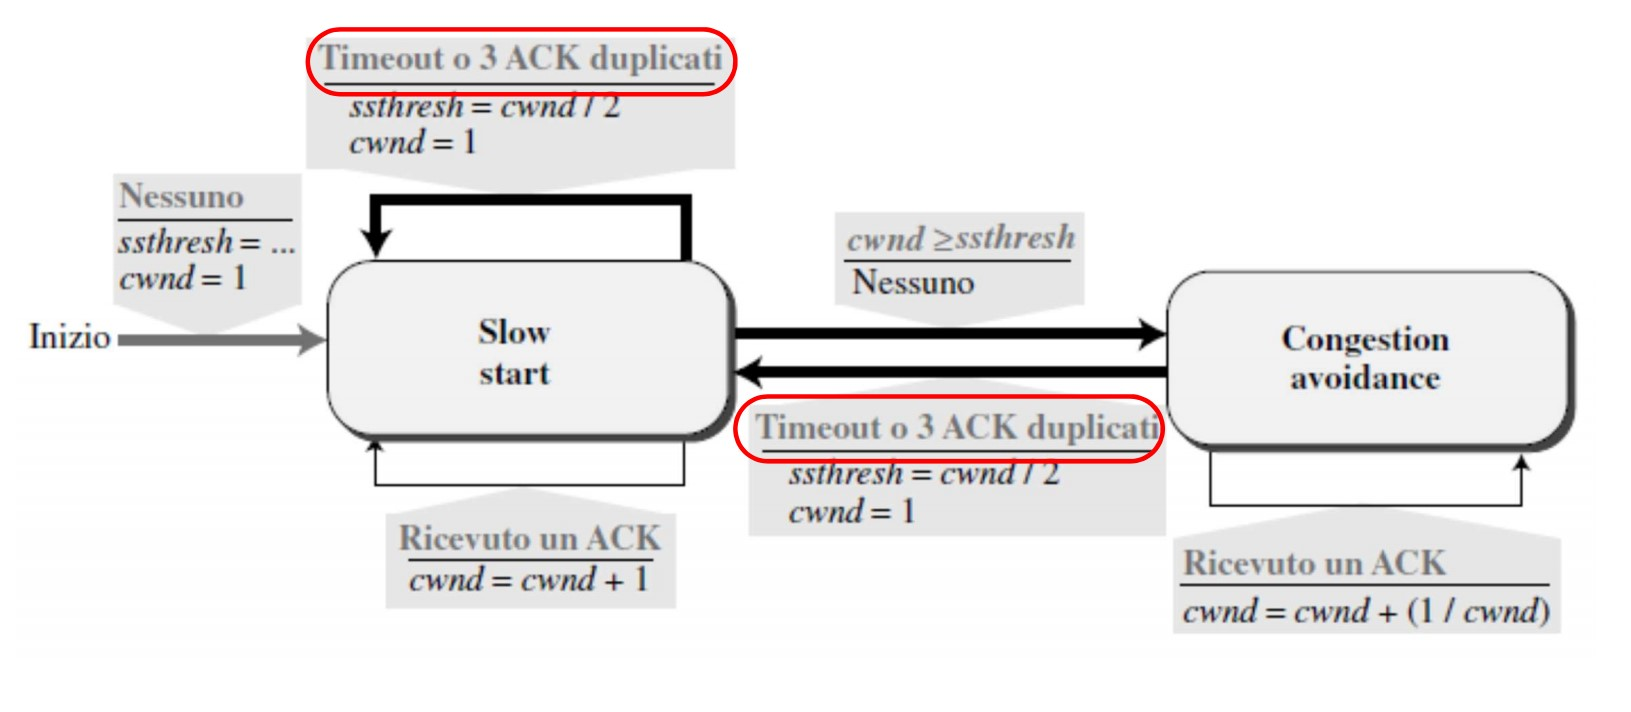
\includegraphics[width=0.8\textwidth]{immagini/TCP_Taho.jpg}
    \caption*{TCP Taho}
\end{figure}

TCP Taho reagisce ai due sintomi di congestione, il timeout e i tre riscontri duplicati, nello stesso modo.\
In questa versione, una volta aperta la connessione, TCP avvia l'algoritmo \emph{slow start} e imposta la variabile \emph{ssthresh} a un valore pre-concordato (solitamente multiplo di MSS) e \emph{cwnd} a 1 MSS.\
In questo stato, come già detto, ogni volta che arriva un riscontro la dimensione della finestra di congestione viene aumentata di 1.\
È evidente che si tratta di una strategia molto aggressiva che incrementa esponenzialmente la dimensione della finestra, cosa che può comportare una congestione.

Se viene rilevata la congestione (scadenza del timeout o ricezione di tre riscontri duplicati), TCP interrompe immediatamente la crescita esponenziale, fa ripartire l'algoritmo slow start con un nuovo threshold uguale alla metà del valore corrente di \emph{cwnd} e reimposta la dimensione della finestra a 1.\
In altri termini, non solo TCP riparte dall'inizio ma aggiorna anche il threshold.\
Se non viene rilevata congestione fino al raggiungimento del threshold, TCP considera di aver raggiunto il massimo delle possibili ambizioni e di non poter continuare a ingrandire la finestra a tale velocità.\
Si sposta quindi nello stato di \emph{congestion avoidance}, dove la dimensione della finestra viene incrementata di 1 ogni volta che viene che riceve un numero di riscontri pari alla dimensione corrente della finestra.\
Si noti che non vi è un limite alla dimensione della finestra che può essere raggiunta in questo stato:\ la crescita lineare continua fino alla chiusura della connessione o fino a quando viene rilevata la congestione.\
Se la congestione viene rilevata in questo stato, TCP reimposta il valore di \emph{ssthresh} alla metà del valore corrente di \emph{cwnd} e si sposta nuovamente nello stato \emph{slow start}.

Sebbene in questa versione di TCP la dimensione di \emph{ssthresh} venga continuamente aggiornata a ogni rilevazione di congestione, essa non diviene necessariamente minore del valore precedente.

\subsubsection{\emph{TCP Reno}}

Questa versione di TCP tratta i due sintomi della congestione, il timeout e la ricezione dei tre riscontri duplicati, in modo differente.\
Quando avviene un timeout, TCP passa allo stato \emph{slow start} (o riparte in questo stato se già vi si trova).\
Quando riceve tre riscontri duplicati, TPC passa allo stato \emph{fast recovery} e vi rimane fintantoché arrivano altri riscontri duplicati.\
Lo stato \emph{fast recovery} è in un certo senso uno stato intermedio fra gli stati \emph{slow start} e \emph{congestion avoidance}.\
Si comporta come lo \emph{slow start}, nel senso che \emph{cwnd} cresce esponenzialmente, ma il valore iniziale di \emph{cwnd} è uguale a \emph{ssthresh} più 3 MSS (anziché 1).\
Quando TCP passa nello stato \emph{fast recovery}, possono avvenire tre eventi principali.\
Se continuano ad arrivare riscontri duplicati, TPC rimane nello stato ma \emph{cwnd} cresce esponenzialmente.\
Se avviene un timeout, TCP assume che vi sia una reale congestione nella rete e passa allo stato \emph{slow start}.\
Se arriva un nuovo riscontro (non duplicato), TCP passa allo stato \emph{congestion avoidance}, ma riduce il valore di \emph{cwnd} al valore \emph{ssthresh} come se i tre riscontri duplicati non fossero stati ricevuti e la transizione fosse dallo stato \emph{slow start} allo stato \emph{congestion avoidance}.

\begin{figure}[H]
    \centering
    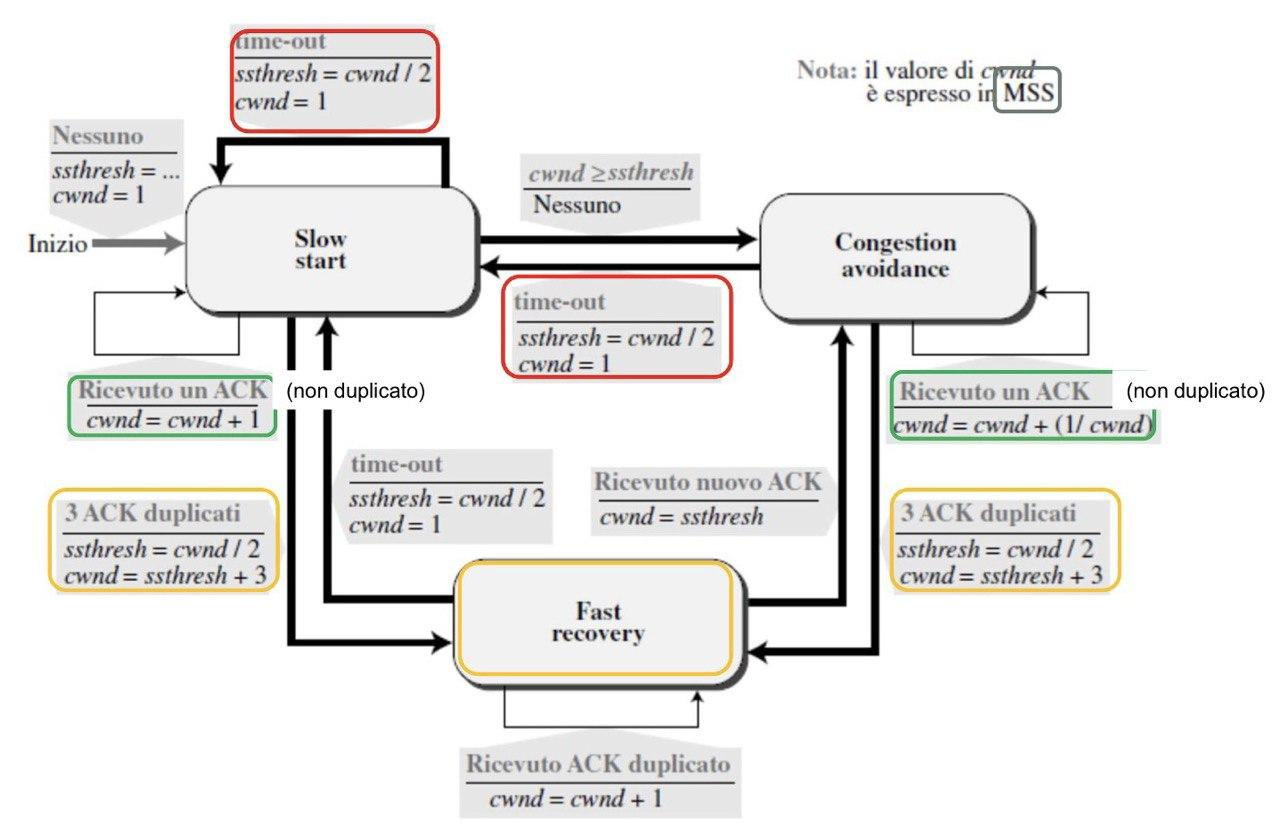
\includegraphics[width=0.7\textwidth]{immagini/TCP_Reno.jpg}
    \caption*{TCP Reno}
\end{figure}

\paragraph{\emph{Additive increase, multiplicative decrease}}

La versione più diffusa di TCP è attualmente la Reno.\
In questa versione si è osservato che nella maggior parte dei casi la congestione viene rilevata e gestita tramite la rilevazione dei tre riscontri duplicati.\
Anche se vi sono alcuni eventi di timeout, TCP recupera rapidamente la situazione grazie alla crescita esponenziale.\
In altri termini, in una connessione TCP di lunga durata, se si ignorano gli stati \emph{slow start} e la breve crescita esponenziale durante il \emph{fast recovery}, la finestra di congestione TCP viene calcolata come $cwnd = cwnd + (1/cwnd)$ quando arriva un riscontro (congestion avoidance) e $cwnd=cwnd/2$ quando viene rilevata la congestione, come se lo \emph{slow start} non esistesse e il \emph{fast recovery} fosse ridotto a zero.\
La prima espressione viene chiamata \emph{incremento additivo} (additive increase), la seconda \emph{decremento moltiplicativo} (multiplicative decrease).\
La dimensione della finestra di congestione, una volta terminata la fase di slow start iniziale, segue un profilo a dente di sega chiamato \emph{AIMD} (Additive Increase, Multiplicative Decrease).

\subsubsection{\emph{Throughput di TCP}}

Il \emph{Throughput} del protocollo TCP dipende dal comportamento della finestra di congestione.\
Esso è facile da calcolare se si assume che \emph{cwnd} sia una funzione costante di RTT:\ con questa ipotesi poco realistica si ha $throughput = cwnd/RTT$, poiché TCP invia \emph{cwnd} byte di dati e ne riceve i riscontri corrispondenti in un tempo RTT.\
Ma il comportamento di TCP non è costante:\ è piuttosto un profilo a denti di sega, con numerosi minimi e massimi relativi.\
Se i denti fossero tutti uguali, potremmo asserire che

\begin{center}
    $throughput = [(massimo+minimo)/2]/RTT$
\end{center}

Sapendo che il valore del massimo è il doppio del valore del minimo poiché a ogni rilevazione di congestione il valore \emph{cwnd} è impostato alla metà del suo valore precedente, il throughput può essere calcolato come

\begin{center}
    $throughput = 0,75 \cdot W_{max}/RTT$
\end{center}
dove W\textsubscript{max} è la dimensione media della finestra quando avviene la congestione.

\pagebreak

\subsubsection{Equità (fairness)}

Ipotesi:\
\begin{itemize}
    \item \textit{K} connessioni TCP insistono su un unico link di capacità \textit{R} bit/s
    \item Le connessioni hanno gli stessi valori di MSS e RTT
    \item Non ci sono altri protocolli che insistono sullo stesso link
\end{itemize}
Risultato:\ Ognuna delle connessioni TCP tende a trasmettere $R/K$ bit/s
\begin{figure}[H]
    \centering
    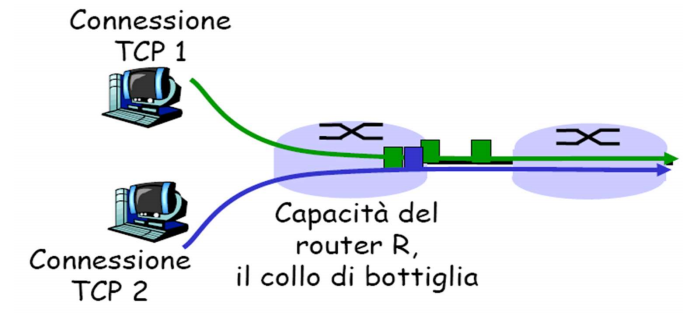
\includegraphics[width=0.6\textwidth]{immagini/Fairness_TCP.png}
\end{figure}

\section{Il protocollo UDP (User Datagram Protocol)}

UDP (User Datagram Protocol) è un protocollo del livello trasporto inaffidabile e privo di connessione.\
Non aggiunge nulla ai servizi di IP eccetto la comunicazione tra processi.\
Per quale motivo un processo dovrebbe utilizzare UDP, se offre così pochi servizi? Gli svantaggi hanno come contropartita alcuni vantaggi.\
UDP è protocollo molto semplice con un overhead (carico aggiuntivo) minimo.\
Se un processo vuole inviare un piccolo messaggio senza doversi preoccupare troppo dell'affidabilità, può utilizzare UDP.\
Inviare un messaggio con UDP richiede meno interazioni fra il mittente e il destinatario rispetto all'impiego del TCP.\
Essendo meno complesso e offrendo meno servizi, è più indicato in contesti dove occorra un completo controllo della temporizzazione (applicazioni time-sensitive come la trasmissione di dati multimediali).

\subsection{Struttura dei datagrammi utente}

I pacchetti UDP sono chiamati \emph{datagrammi utente}; la loro intestazione è costituita da 4 campi di 2 byte (16 bit) per un totale di 8 byte fissi.\
I primi due campi definiscono i numeri di porta di mittente e destinatario.\
Il terzo campo definisce la lunghezza totale, intestazione più dati, del datagramma utente.\
I 16 bit possono definire una lunghezza totale da 0 a 65535 byte, ma in realtà la dimensione è inferiore perché il datagramma utente UDP viene inserito in un datagramma IP con lunghezza totale di 65535 byte.\
L'ultimo campo può contenere il checksum opzionale.

\subsection{Servizi UDP}

UDP fornisce il servizio di \emph{comunicazione tra processi} utilizzando i socket address (indirizzo IP + numero di porta), ed eseguendo il \emph{multiplexing e demultiplexing} dei pacchetti.\
Il concetto di numero di porta è già stato introdotto e utilizzato, ma non si è detto nulla a proposito come le porte vengano realizzate.\
L'idea di base, usata nel protocollo UDP, è quella di coda.\
Quando un processo client viene avviato richiede al sistema operativo la disponibilità di una porta.\
Il sistema operativo crea due code, una d'ingresso e una d'uscita, associate al processo.\
In alcuni sistemi operativi viene creata la sola coda d'ingresso.

Il protocollo UDP, per inviare un messaggio da un processo a un altro, \emph{incapsula} e \emph{decapsula} il messaggio.\
Tuttavia la comunicazione tra processi realizzata da UDP è \emph{priva di connessione}, il che vuol dire che ogni datagramma viene trasmesso in modo indipendente dagli altri.\
Non esiste alcuna relazione tra i datagrammi anche nel caso in cui essi provengano dallo stesso processo mittente e siano indirizzati allo stesso processo destinatario.\
Il fatto che i datagrammi utente non vengano numerati e che la trasmissione avvenga senza apertura e chiusura di una connessione, risulta in una totale indipendenza dei percorsi seguiti dai vari datagrammi.

Una delle conseguenze della trasmissione senza connessioni è che il processo mittente non può inviare un flusso di dati al protocollo UDP e aspettarsi che questi lo suddivida in datagrammi correlati.\
I processi devono inviare all'UDP richieste di dimensioni sufficientemente piccole da poter essere inserite ciascuna in un singolo datagramma utente; solo i processi che usano messaggi di piccole dimensioni, inferiori a 65507 byte (65535 meno gli 8 byte per l'intestazione UDP e 20 byte per l'intestazione IP) possono utilizzare il protocollo UDP.

Il protocollo UDP è un protocollo di trasporto estremamente semplice.\
Non vi è alcun controllo del flusso e quindi nessun meccanismo di finestre scorrevoli:\ il destinatario può quindi trovarsi in situazione di congestione.\
L'assenza di controllo di flusso implica che siano i processi che usano UDP, se necessario, a dover fornire questo servizio.

Inoltre, essendo UDP un protocollo privo di connessione, non fornisce alcun controllo della congestione.\
UDP è nato per applicazioni che inviano pacchetti in maniera sporadica e di dimensione limitate:\ non potrebbero quindi creare congestione nella rete.\
Questa ipotesi può non essere sempre verificata nelle applicazioni moderne, dove UDP viene utilizzato per il trasferimento di audio e video in tempo reale.

Riguardo al controllo degli errori, l'unico meccanismo in UDP è il checksum; al mittente, quindi, non viene notificata la perdita o l'eventuale duplicazione di un messaggio.\
In caso di errore evidenziato dal checksum il destinatario elimina il pacchetto ma non invia alcuna notifica.\
A questa carenza del protocollo UDP devono inevitabilmente sopperire i processi che lo impiegano.

\subsubsection{\emph{Checksum}}

Il checksum in UDP riguarda tre parti:\ pseudoheader, intestazione e dati provenienti dal livello applicazione.\
Lo \emph{pseudoheader} è una parte dell'intestazione del pacchetto IP in cui viene incapsulato il datagramma utente, con alcuni dei campi impostati a zero.

\begin{figure}[H]
    \centering
    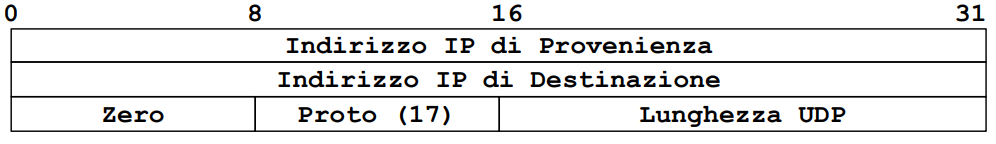
\includegraphics[width=0.8\textwidth]{immagini/Pseudoheader.png}
    \caption*{Pseudoheader – usato per calcolo checksum}
\end{figure}

Se il checksum non includesse lo pseudoheader, il datagramma utente, pur non avendo subito danni durante la trasmissione, potrebbe finire all'host sbagliato per via di errori nel pacchetto IP che lo trasporta.\
Il campo protocollo permette di distinguere tra i pacchetti UDP e quelli TCP.\
Se i processi possono usare entrambi questi protocolli, i numeri di porta possono essere gli stessi.\
Il valore del campo protocollo corrispondente all'UDP è 17; se tale valore viene modificato durante la trasmissione, il calcolo del checksum evidenzia questa anomalia e UDP scarta il pacchetto.\
I pacchetti quindi non rischiano di essere consegnati al protocollo sbagliato.

\paragraph{Calcolo del checksum}

\begin{itemize}
    \item Mittente
          \begin{itemize}
              \item Campo checksum a 0
              \item Tratta il contenuto del datagramma UDP come una sequenza di parole da 16 bit
              \item Checksum:\ somma le parole di 16 bit in complemento a uno
              \item Complemento a uno del risultato della somma
              \item Il mittente pone il valore della checksum nel campo del checksum del datagramma UDP
          \end{itemize}
    \item Ricevente
          \begin{itemize}
              \item Calcola la checksum del segmento ricevuto
              \item Se il valore del checksum è diverso da 0 allora è stato rilevato un errore e il messaggio viene scartato.
          \end{itemize}
\end{itemize}

\begin{figure}[H]
    \centering
    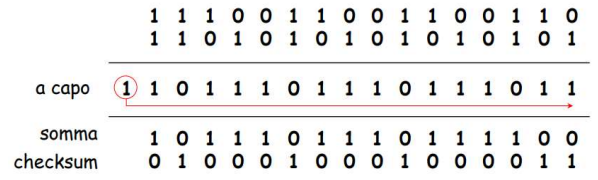
\includegraphics[width=0.7\textwidth]{immagini/Checksum.png}
    \caption*{Calcolo del checksum}
\end{figure}

